\section{Giới thiệu}

Phân đoạn ngữ nghĩa là bài toán gán nhãn cho từng pixel trong ảnh đầu vào, trong đó mô hình phải đồng thời nắm bắt ngữ cảnh toàn cục và bảo toàn các tín hiệu cục bộ. Về mặt hình thức, với ảnh đầu vào $ \mathbf{X} \in \mathbb{R}^{H \times W \times 3}$ mục tiêu là dự đoán bản đồ nhãn $ \mathbf{Y} \in \{1,2,\dots,K\}^{H \times W} $ trong đó $H, W$ là kích thước ảnh và $K$ là số lớp cần phân đoạn. Thiết lập này đặc biệt quan trọng trong các hệ thống theo dõi dinh dưỡng, bếp thông minh, robot chế biến và kiểm soát chất lượng thực phẩm, nơi yêu cầu về độ chính xác phải đi kèm với khả năng suy luận hiệu quả trong thực tế \cite{mahalik2010trends, stemmer2018vision, gao2019smartfridge, wang2019smartrefrigerator}.

Trong miền ảnh thực phẩm, bài toán trở nên khó hơn đáng kể vì mỗi pixel không chỉ cần được gán đúng nhãn ngữ nghĩa, mà còn phải được tách khỏi các thành phần nguyên liệu lân cận có hình thái và màu sắc gần nhau. Các thành phần này thường chồng lấp, có ranh giới mờ, biến đổi mạnh theo cách chế biến và mang tính fine-grained rõ rệt. Do đó, chất lượng phân đoạn không chỉ phụ thuộc vào khả năng mô hình hóa ngữ cảnh, mà còn phụ thuộc mạnh vào việc giữ được biên, texture và cấu trúc bề mặt như những tín hiệu phân biệt cục bộ then chốt.

FoodSeg103 là benchmark tiêu biểu cho thiết lập ingredient-level này \cite{benchmarkfood}. Tuy nhiên, đây cũng là một benchmark khó: số lớp lớn, biến thiên nội lớp cao, tương đồng liên lớp mạnh, phân bố đuôi dài nghiêm trọng và mỗi ảnh thường chứa nhiều nguyên liệu cùng lúc. Những đặc tính đó khiến mô hình dễ thiên lệch về lớp phổ biến, làm mịn ranh giới và bỏ sót các lớp hiếm, đặc biệt khi kiến trúc không đủ nhạy với local detail.

\begin{figure}[H]
    \centering
    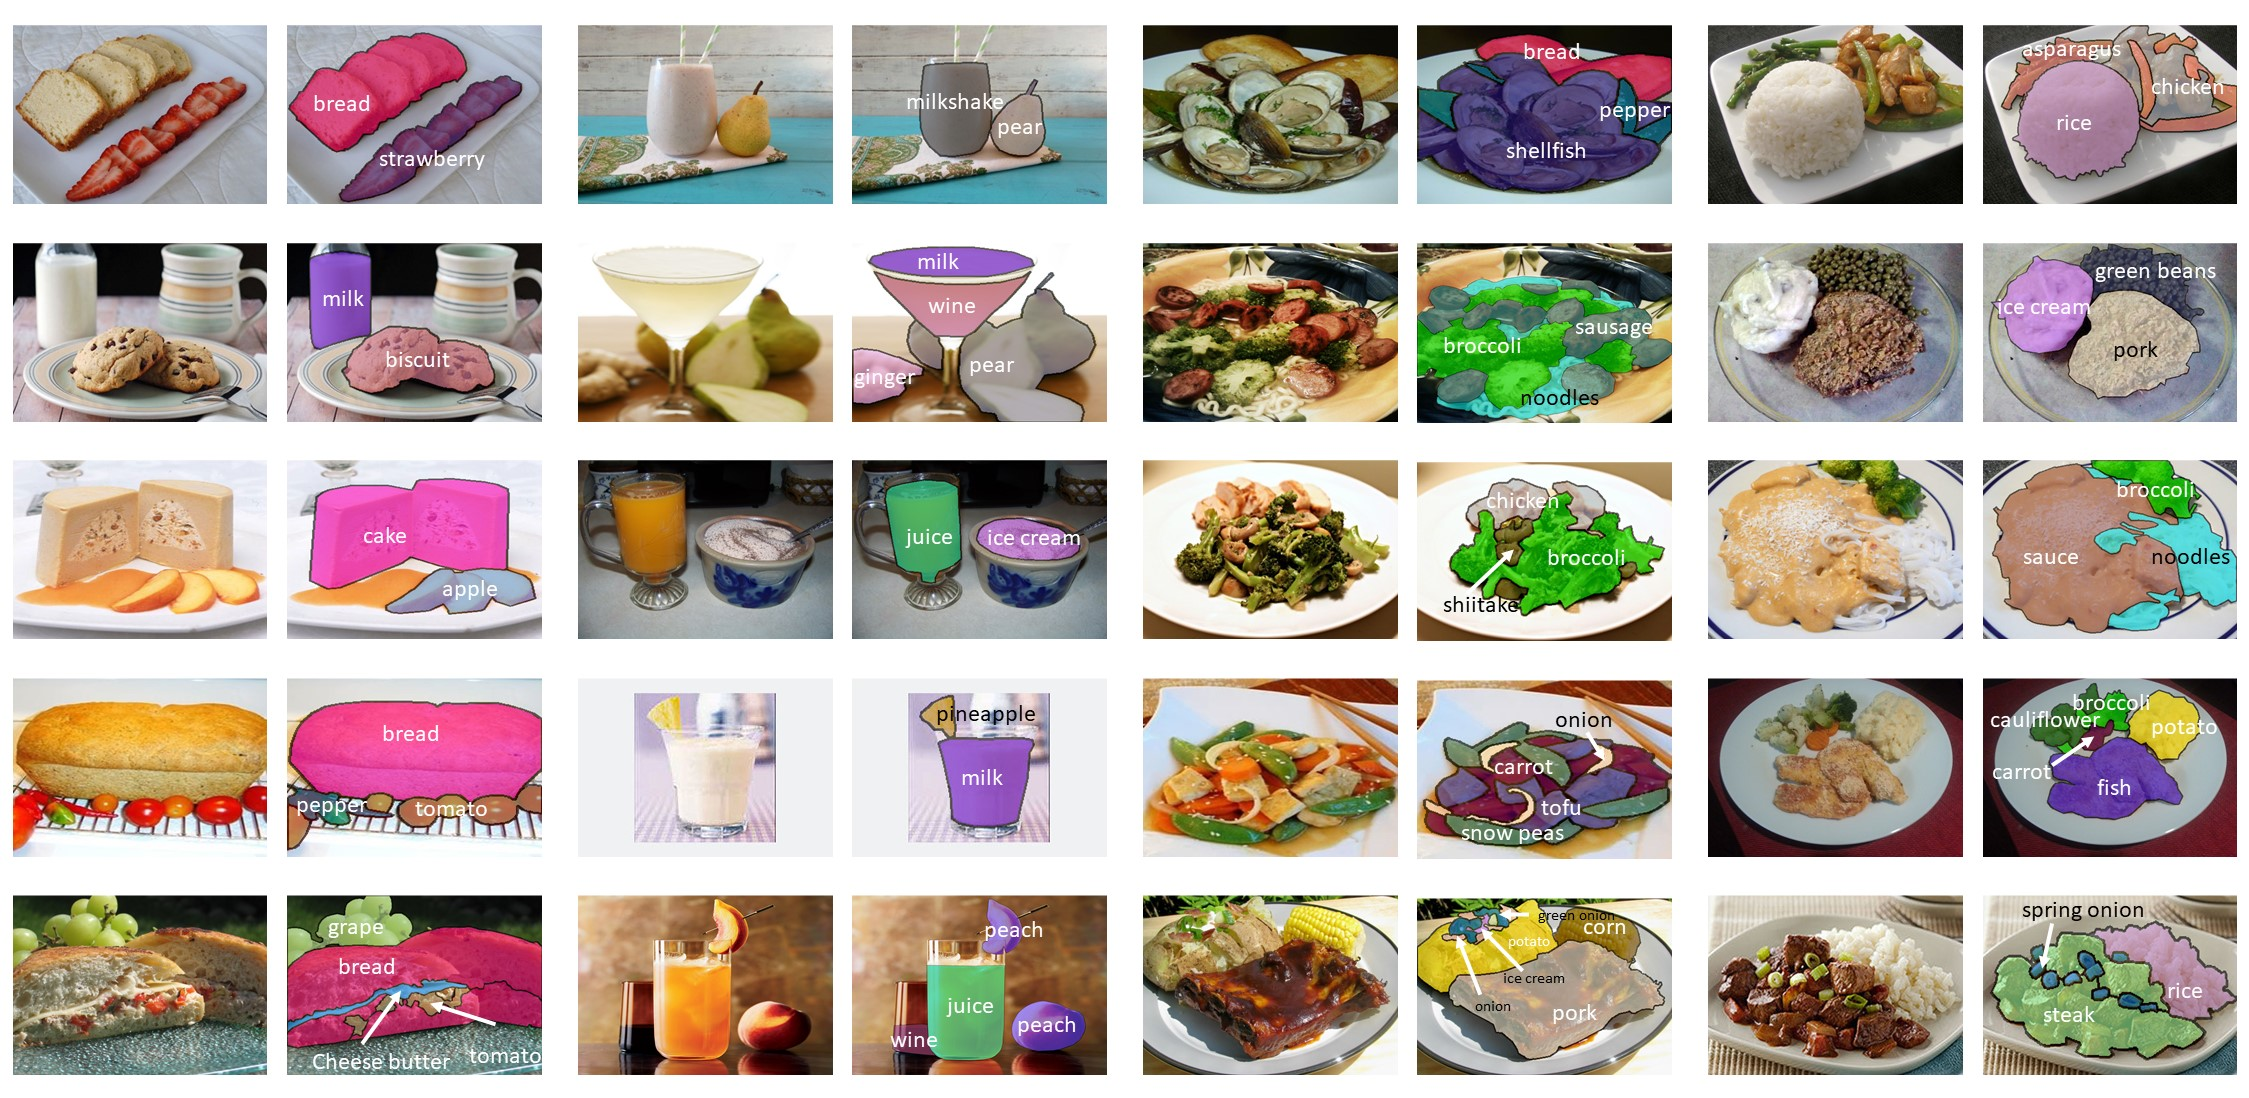
\includegraphics[width=\linewidth]{img/foodseg103.png}
    \caption{Mẫu ảnh đại diện của FoodSeg103, cho thấy độ đa dạng cao về texture, màu sắc và trạng thái bề mặt giữa các nguyên liệu.}
\end{figure}

Vấn đề nghiên cứu vì thế nằm ở sự đánh đổi giữa độ chính xác và hiệu quả suy luận. Các mô hình segmentation mạnh giàu ngữ cảnh có thể cho kết quả tốt hơn nhưng thường đòi hỏi chi phí tính toán cao, khó triển khai trên thiết bị tài nguyên hạn chế. Ngược lại, các kiến trúc lightweight đạt tốc độ cao nhờ downsample sớm và nén biểu diễn, nhưng chính chiến lược đó có thể làm suy giảm các đặc trưng cục bộ quan trọng đối với ảnh thực phẩm fine-grained. Trong bối cảnh đó, nghiên cứu hiện tại được định vị như một \textbf{baseline study}: thay vì tuyên bố đã giải quyết hoàn chỉnh bài toán texture-aware lightweight segmentation, báo cáo tập trung chuẩn hóa baseline BiSeNet trực tiếp trên FoodSeg103 nguyên thủy làm mốc tham chiếu cho các cải tiến texture/local-detail-aware ở giai đoạn tiếp theo.

Từ định vị đó, báo cáo tập trung vào ba đóng góp chính:
\begin{itemize}[leftmargin=1.5em]
    \item Phân tích định lượng bộ dữ liệu FoodSeg103 để chỉ ra các khó khăn cốt lõi của bài toán, bao gồm long-tail imbalance, chồng lấp thành phần, ranh giới yếu và chênh lệch độ phân giải giữa các split.
    \item Thiết lập và chuẩn hóa baseline BiSeNet trên không gian nhãn nguyên thủy 103 lớp để tạo mốc tham chiếu công bằng cho các nghiên cứu texture-aware lightweight segmentation tiếp theo.
    \item Tổ chức thực nghiệm mở rộng về tái cấu trúc không gian nhãn (103 xuống 75) để phân tích bổ sung ảnh hưởng của phân mảnh nhãn, tách biệt với baseline chính.
\end{itemize}

\subsection{Phát biểu bài toán}

Bài toán phân đoạn ngữ nghĩa (\textit{semantic segmentation}) là bài toán gán nhãn ngữ nghĩa cho từng điểm ảnh trong ảnh đầu vào. Với một ảnh đầu vào
\[
\mathbf{X} \in \mathbb{R}^{H \times W \times 3},
\]
mục tiêu là dự đoán một bản đồ nhãn
\[
\mathbf{Y} \in \{1,2,\dots,K\}^{H \times W},
\]
trong đó $H, W$ lần lượt là chiều cao và chiều rộng của ảnh, còn $K$ là số lớp cần phân đoạn.

Trong bài toán phân đoạn ảnh thực phẩm ở mức nguyên liệu, mỗi pixel cần được gán vào một lớp nguyên liệu tương ứng, ví dụ như \textit{rice}, \textit{beef}, \textit{lettuce}, \textit{tomato}, \dots Với mô hình học sâu, mạng nhận ảnh đầu vào $\mathbf{X}$ và sinh ra tensor logit
\[
\mathbf{Z} \in \mathbb{R}^{H \times W \times K},
\]
trong đó $\mathbf{Z}_{i,j,c}$ biểu diễn điểm số chưa chuẩn hóa của lớp $c$ tại pixel $(i,j)$. Xác suất dự đoán cho lớp $c$ tại pixel $(i,j)$ được tính bằng hàm softmax:
\[
p_{i,j,c} = \frac{\exp(\mathbf{Z}_{i,j,c})}{\sum_{k=1}^{K} \exp(\mathbf{Z}_{i,j,k})}.
\]

Nhãn dự đoán cuối cùng tại pixel $(i,j)$ được xác định bởi:
\[
\hat{y}_{i,j} = \arg\max_{c \in \{1,\dots,K\}} p_{i,j,c}.
\]

Như vậy, bài toán phân đoạn ngữ nghĩa có thể xem là bài toán phân lớp đa lớp ở mức pixel, trong đó mô hình phải đồng thời học được ngữ cảnh toàn cục và bảo toàn các chi tiết cục bộ như biên, texture và cấu trúc bề mặt để phân biệt các lớp có mức độ tương đồng thị giác cao.

\subsection{Hàm mất mát}

Trong nghiên cứu này, mô hình được huấn luyện bằng hàm mất mát \textit{pixel-wise cross-entropy}. Gọi $y_{i,j}$ là nhãn thật tại pixel $(i,j)$, khi đó hàm mất mát trên toàn ảnh được viết là:
\[
\mathcal{L}_{\mathrm{CE}}
=
-\frac{1}{|\Omega|}
\sum_{(i,j)\in\Omega}
\log p_{i,j,y_{i,j}},
\]
trong đó $\Omega$ là tập các pixel hợp lệ được dùng để huấn luyện, và $|\Omega|$ là số lượng pixel trong tập này.

Viết tường minh theo đầu ra softmax, ta có:
\[
\mathcal{L}_{\mathrm{CE}}
=
-\frac{1}{|\Omega|}
\sum_{(i,j)\in\Omega}
\log
\left(
\frac{\exp(\mathbf{Z}_{i,j,y_{i,j}})}
{\sum_{c=1}^{K}\exp(\mathbf{Z}_{i,j,c})}
\right).
\]

Hàm mất mát này buộc mô hình tăng xác suất cho lớp đúng tại từng pixel. Trong thực tế, nếu dữ liệu có mất cân bằng lớp mạnh, có thể mở rộng sang \textit{weighted cross-entropy}; tuy nhiên, dạng cơ sở được sử dụng trong báo cáo này là cross-entropy chuẩn ở mức pixel.

\subsection{Các chỉ số đánh giá}

Để đánh giá chất lượng phân đoạn, báo cáo sử dụng ba chỉ số chính: \textbf{mIoU}, \textbf{mAcc} và \textbf{aAcc}. Gọi $TP_c$, $FP_c$, $FN_c$ lần lượt là số pixel đúng dương, dương giả và âm giả của lớp $c$, khi đó:
\[
\mathrm{mIoU}=\frac{1}{K}\sum_{c=1}^{K}\frac{TP_c}{TP_c+FP_c+FN_c},
\]
\[
\mathrm{mAcc}=\frac{1}{K}\sum_{c=1}^{K}\frac{TP_c}{TP_c+FN_c},
\]
\[
\mathrm{aAcc}=\frac{\sum_{c=1}^{K}TP_c}{\sum_{c=1}^{K}(TP_c+FN_c)}.
\]

Trong đó, mIoU phản ánh mức giao nhau trên hợp trung bình giữa dự đoán và ground truth theo từng lớp, mAcc phản ánh độ chính xác trung bình theo lớp, còn aAcc phản ánh độ chính xác toàn cục trên toàn bộ pixel. Với bài toán phân đoạn thực phẩm có mất cân bằng lớp, mIoU vẫn được xem là chỉ số chính để so sánh mô hình.